\documentclass[sigconf]{acmart}

\settopmatter{printacmref=false}
\renewcommand\footnotetextcopyrightpermission[1]{}


%%
%% \BibTeX command to typeset BibTeX logo in the docs
\AtBeginDocument{%
  \providecommand\BibTeX{{%
    Bib\TeX}}}

%% These commands are for a PROCEEDINGS abstract or paper.
\acmConference[APE CS 598]
{APE CS 598}{Spring 2025}{Urbana, IL}

\begin{document}

\title{Java Chess Engine}

\author{Adam McNeil}
\email{adamwm4@illinois.edu}
\affiliation{%
  \country{University of Illinois Urbana-Champaign, Urbana, Illinois, USA}
}


\begin{abstract}
In this paper, we highlight the optimizations performed on a Java chess engine.
The goal of these optimizations is to increase the depth that the engine can compute in a reasonable time (approx. 1 sec).
Although this does not necessarily make it better at playing chess since we are computing at a small depth, increasing it will make the chess engine more accurate.
There are also other ways to improve the chess engine, but they are not the focus of this paper.
\end{abstract}

\maketitle
Link to the engine: \url{https://github.com/adamMcneil/chess-engine}

Link to the bot: \url{https://github.com/adamMcneil/cheeky-koala-lichess-bot}
\section{Background}
This project was originally developed by me and a friend in the summer of 2021.
We designed it in an object-oriented way, which was not always the most performant.
This is the original file structure of the project:
\begin{verbatim}
Cheakykoala/
|-- Pieces/
|   |-- Bishop.java
|   |-- Empty.java
|   |-- King.java
|   |-- Knight.java
|   |-- Pawn.java
|   |-- Piece.java
|   |-- Queen.java
|   |-- Rook.java
|-- Board.java
|-- Color.java
|-- Main.java
|-- Move.java
|-- Position.java
|-- PromotionMove.java
\end{verbatim}
\texttt{Piece} is an abstract class that the other pieces inherit from.
\texttt{Color} is an \texttt{Enum} with three values: \texttt{w}, \texttt{b}, and \texttt{g}.
These represent white, black, and gray, respectively.
Gray is used for the Empty Piece. Having an Empty Piece to represent a blank square does not seem very performant, but, surprisingly, it does not make a huge impact on performance.
The \texttt{Position} class adds a lot of overhead to the program; all it does is wrap two integers together to represent the position.
It introduces a lot of unnecessary object allocation and function calls.
\texttt{PromotionMove} inherits from the \texttt{Move} class; this is probably not the best way to handle this and should be optimized.

\subsection{Gradle}
In the past, I relied on the IntelliJ IDE for building the project.
Since the project was out of date, it did not work when I build the project.
So, I decided to switch to Gradle for building the project.
This was a good decision because it offers a lot of different actions out of the box, like: running the application, running tests, and generating jar files.

\subsection{IntelliJ}
Since I am a student, I have access to IntelliJ Ultimate. IntelliJ Ultimate offers a lot of features that will be very helpful for performance engineering.
They have a built-in code coverage tool that will show what percentage of lines are covered by your tests.
They also give you access to a profiling program that will generate a Flame Graph, Call Tree, Method List, Timeline, CPU Usage, and Events.
It also gives me access to the debugger, which will be helpful for debugging.

\subsection{Lichess}
I used an open-source resource \cite{lichess-bot} to connect my chess engine to Lichess.
It uses the universal chess interface (UCI) \cite{uci} to talk to Lichess.
In order to use the program, you only need to point the program to your chess engine executable that responses to a simple API.
To communicate with Lichess, you must make your chess engine respond to very simple inputs described in Table~\ref{tab:api}.
You can use a YAML config file to configure your chess engine.
It also allows you to use opening books, which are a set of games that the engine will play by default at the beginning of a game \cite{pgn}.

In order to turn the chess project into an executable, I use Gradle to build the project into a jar file and then use a bash script to execute the file.
This just runs the Java interpreter.
We use the following simple script to run the program.
\begin{verbatim}
#!/bin/bash
java -cp chess-engine-1.0-SNAPSHOT.jar cheekykoala.Main
\end{verbatim}

\begin{table*}[h]
    \centering
    \renewcommand{\arraystretch}{1.2}
    \setlength{\tabcolsep}{8pt}
    \begin{tabular}{|c|c|c|}
        \hline
        \textbf{Input} & \textbf{Description} & \textbf{Output} \\
        \hline
        \texttt{uci} & Confirming that the engine is running UCI. & \texttt{uciok} \\
        \hline
        \texttt{isready} & Confirming that the engine is ready. & \texttt{readyok} \\
        \hline
        \texttt{position <fen> moves <list of moves>} & Load the board position from the server & \\
        \hline
        \texttt{go wtime <n> btime <n> winc <n> binc <n>} & Output a move that you want to make. & bestmove (e2e4) \\
        \hline
        \texttt{quit} & \texttt{Quit the chess engine} & \\
        \hline
    \end{tabular}
    \caption{A description of the API that the chess engine needs to respond to play on Lichess.}
    \label{tab:api}
\end{table*}


\section{Introduction}
A chess engine consists of a couple of basic parts:
\begin{enumerate}
    \item \textbf{Move Generation} – Responsible for determining all legal moves from a given board state.
    \item \textbf{Board Evaluation} – Assigns a score or value to a position to help judge its quality.
    \item \textbf{Search Algorithm} - Combines the other components to find the best move in any given state.
\end{enumerate}

\subsection{Move Generation}
This is relatively simple; it just requires you to specify the rules of chess in a programming language.
This requires a lot of testing and debugging to cover all of the corner cases (literally the corner cases).
However, the structure of the data that you use in this case will affect how efficiently you can produce a list of legal moves.
One of the main trade-offs that we found was increasing the size of dat stored and recomputing values.

\subsection{Board Evaluation}
This in its simplest form is a variable with four possible values:
\begin{itemize}
    \item Black in checkmate
    \item White in checkmate
    \item Stalemate
    \item None
\end{itemize}
However, this is an unrealistic metric because the search space is too massive to find a checkmate from the starting position, and the bot would see no way to win, so it would play randomly.

So we can use the pieces on the board as a heuristic for who is in a better position.
The next obvious metric would be material advantage (this is simply who has better pieces on the board).
We assign values to each piece and make the black pieces the negative value of the white pieces.
In this way, we can have the player prefer positions where they have better/more pieces on the board and the other person has worse/fewer pieces on the board.
This is the most common heuristic for who is winning a game.

However, this does not capture everything that chess players use to determine which side is in a better position.
Players also develop pieces; this usually means moving pieces toward the center of the board or having a good pawn structure.
To capture this, we can use a table of values that offer a little benefit to pieces in each of those good positions.
Each Piece has a separate table of values that is used to determine the benefit of each Piece in a specific location on the board.
Intuitively, this is because it is better to have your king in the back protected, and for pawns, it is good to have them on the second to last row so that they are close to promotion.

\subsection{Move Search}
Since chess is a two-player game, it uses a mini-max algorithm to find the best move.
There are better explanations of this algorithm online somewhere, but at a basic level, the computer takes turns maximizing and minimizing the branching board state.
This simulates both players playing optimally and will allow the computer to compute the most optimal solution.

Now that we have a move generator and a way to compare boards, we can use standard graph algorithms to search for the best move.
The most basic search would be a depth search.
However, this is not optimal in chess because the player needs to move in real time.
It is hard to know how long the depth search will take.
Because of this, it is hard to determine the depth that the bot should search.
Furthermore, the search needs to be completed before it returns a move.

The algorithm that is best for looking for moves in chess is iterative deepening.
It works by doing consecutive executions of a depth search.
This allows the bot to return the best move of the deepest depth it has computed.
Since the small depth happen very quickly it always has a move to return.

\section{Related Works}
Stockfish \cite{stockfish} is the state of the art in chess engines today.
It has dominated the Top Chess Engine Championship for the past several years \cite{stockwiki}.
It is implemented with C++ and is open source.

The project uses a distributed testing framework called Fishtest, where people donate CPU time to play games against the release of Stockfish.
After playing a bunch of games, they determine if the change was better and should be kept \cite{stockwiki}.
Stockfish is trying to optimize winning games; this is not what we are trying to optimize in this paper.
This paper primarily focuses on being able to compute a larger depth faster.

It also uses bit boards to represent the state of the board \cite{stockwiki}.
Bit boards work by represent the board with a 64 bits \cite{bitboard}.
Each piece can have a bit board associated with it.
These bit board can be combined to find moves.

One notable change to Stockfish happened in 2020 when they added a neural network (NNUE) to evaluate the state of the board \cite{chesswiki}.
This replaced the heuristics that were previously used to compare boards.

For parallel search it is standard to use the algorithm outlined here \cite{parallel}.
The main challenge of parallelism is using it in conjunction with alpha beta pruning.
Alpha beta pruning depends heavily on the order the nodes are searched in, so if they are searched in parallel you cannot control what order to search them in.
It works by computing the "killer move" or the move with the highest heuristic first and then using the rest of the compute power to compare with that move.
Since the heuristic in most chess engine are very good it is able to find the best move very quickly.

\section{Overview}
We perform a wide range of optimizations on the chess engine.
However, all the changes that we made can be categorized into three main groups:
\begin{enumerate}
    \item Data Structure Changes
    \item Parallelism
    \item Search Heuristics
\end{enumerate}

\subsection{Data Structure Changes}
This type of optimization included changing the way we represented the board.
The original optimization used a 2-D array; however, we found that a 1-D array was more efficient.
It reduced overhead by eliminating the Position class and allowed us to identify a position with just an integer.
We were also able to make all of the Piece classes Singleton classes by removing the position variable on the Piece class.
It also included caching computed values so that they do not need to be recomputed.

\subsection{Parallelism}
This type of graph search is highly parallelizable because we can have multiple threads working on different portions of the tree.
The parallelism that we implement in this work parallels the base layer of the mini-max.
Effectively meaning that each of the moves at depth one are being computed in parallel.
Though this does increase the efficiency of the program by a lot, this is not the best way to implement parallelism and leads to a lot of problems that will be discussed in the Implementation section.

\subsection{Search Heuristics}
The mini-max algorithm depends a lot on the order the moves are searched in this is because it uses alpha beta pruning.
By sorting the moves we can prune more branches of the tree.
Additionally, we can take advantage of alpha-beta pruning by creating a list of pseudo moves that included illegal moves but would be likely pruned out because they left the player in a losing position.
Though we are searching over more moves it is much fast to generate the moves and alpha beta pruning becomes more affective.

There are also a lot more optimizations/refactoring that cannot all be reported.
For example, the static arrays were being reallocated in a loop while generating moves, which was causing overhead.
We were also able to restructure if statements to break earlier.

\section{Implementation}
\subsection{Tests}
It is very important to run tests to verify that your application is correct after refactoring for performance.
To achieve this, I used a database of chess positions \cite{jones} and the number of legal moves at a certain depth to verify the accuracy of the chess engine.
Each of the individual tests is formed like the following JSON object.
The test imports the FEN \cite{fen} string and verifies that the number of nodes is the same at that depth of search.
\begin{verbatim}
  {
    "depth":1,
    "nodes":8,
    "fen":"r6r/1b2k1bq/8/8/7B/8/8/R3K2R b KQ - 3 2"
  }
\end{verbatim}
I also created similar tests that would test the piece individually, which would make it easier to pinpoint bugs.
However, when there are bugs at the six levels deep in the move generation it is hard to pin point the bug.
I used the testing methodology outlined in this article \cite{testing}.
It used the divide function ROCE chess engine to pin point the sequence of moves where the bug was.

\subsection{Board Representation} \label{sec:board}
A large refactoring that will increase the efficiency of the program by a lot is representing the board with a 1-D array instead of a 2-D array.
This makes computing moves a little trickier, but it will result in being able to get rid of the \texttt{Position} class.
The \texttt{Position} class is creating a lot of unnecessary object allocations.
The class only contains an \texttt{int[]} with two elements.
By switching to a 1D array to represent the board, we can represent a position on the board with just an \texttt{int}.
\begin{table}[H]
    \renewcommand{\arraystretch}{1.5}
    \setlength{\arrayrulewidth}{1pt}
    \setlength{\tabcolsep}{4pt}
    \begin{tabular}{|c|c|c|c|c|c|c|c|}
        \hline
        0,0  & 1,0  & 2,0  & 3,0  & 4,0  & 5,0  & 6,0  & 7,0  \\
        \hline
        0,1  & 1,1  & 2,1  & 3,1  & 4,1  & 5,1  & 6,1  & 7,1  \\
        \hline
        0,2  & 1,2  & 2,2  & 3,2  & 4,2  & 5,2  & 6,2  & 7,2  \\
        \hline
        0,3  & 1,3  & 2,3  & 3,3  & 4,3  & 5,3  & 6,3  & 7,3  \\
        \hline
        0,4  & 1,4  & 2,4  & 3,4  & 4,4  & 5,4  & 6,4  & 7,4  \\
        \hline
        0,5  & 1,5  & 2,5  & 3,5  & 4,5  & 5,5  & 6,5  & 7,5  \\
        \hline
        0,6  & 1,6  & 2,6  & 3,6  & 4,6  & 5,6  & 6,6  & 7,6  \\
        \hline
        0,7  & 1,7  & 2,7  & 3,7  & 4,7  & 5,7  & 6,7  & 7,7  \\
        \hline
    \end{tabular}
    \caption{This table represents the old indexing scheme used with a 2D array representing the board.}
    \label{tab:example_table}
\end{table}

\begin{table}[H]
    \renewcommand{\arraystretch}{1.5}
    \setlength{\arrayrulewidth}{1pt}
    \setlength{\tabcolsep}{5pt}
    \begin{tabular}{|c|c|c|c|c|c|c|c|}
        \hline
        0  & 1  & 2  & 3  & 4  & 5  & 6  & 7  \\
        \hline
        8  & 9  & 10  & 11  & 12  & 13  & 14  & 15  \\
        \hline
        16  & 17  & 18  & 19  & 20  & 21  & 22  & 23  \\
        \hline
        24  & 25  & 26  & 27  & 28  & 29  & 30  & 31  \\
        \hline
        32  & 33  & 34  & 35  & 36  & 37  & 38  & 39  \\
        \hline
        40  & 41  & 42  & 43  & 44  & 45  & 46  & 47  \\
        \hline
        48  & 49  & 50  & 51  & 52  & 53  & 54  & 55  \\
        \hline
        56  & 57  & 58  & 59  & 60  & 61  & 62  & 63  \\
        \hline
    \end{tabular}
    \caption{This table represents the new indexing scheme used with a 1-D array representing the board.}
    \label{tab:example_table}
\end{table}

We also considered using a BigInteger to represent the state of the board.
But instead of using 1 bit to represent a piece we used 4 bits.
We then could use or, and, and shift operations to store the state of the board.
This was thought to decrease the time to copy the Board class when branching.
However, making this change decreases the efficiency so it was rejected.

\subsection{Caching Board Evaluation}
When keeping track of the evaluation of the board, the simplest scheme is to recompute the evaluation of the board each time it is needed.
This is a linear scan of the board.
We can obviously do better than this by just creating a variable on the board class to store the evaluation by doing this we can create it in constant time.
Storing the evaluation of the board does cause overhead when coping board but the benefit far out way the draw backs.

\begin{figure}[H]
    \centering
    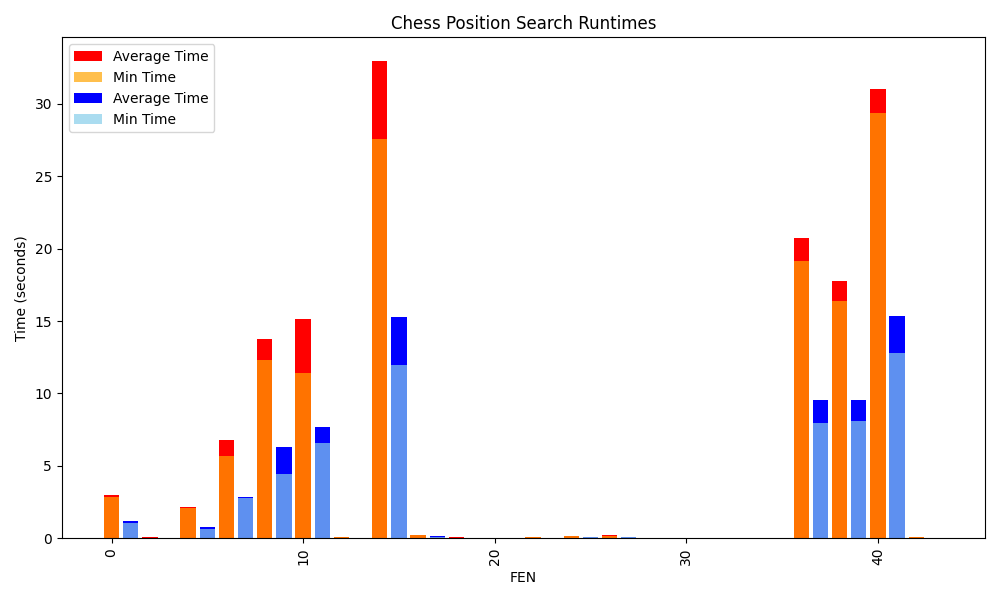
\includegraphics[width=1\linewidth]{recompute-eval-graph.png}
    \caption{The red bars represent the program where the board evaluation was recomputed each time during a depth search. The blue bars are when we cache and update the board evaluation}
    \label{fig:eval-speedup}
\end{figure}

\subsection{Caching Move Type}
For most of the moves in chess, you just move your piece to an empty square or take the piece at that square.
However, some moves require extra logic to perform and detect (e.g. castling, en passant, and promotions).
We did have methods that given a move would tell you what type of move it was but since that information is known when you create the move and is static we can cache it in the Move class.
Though the performance was modest for some benchmarks it made a significant difference.
\begin{figure}[H]
    \centering
    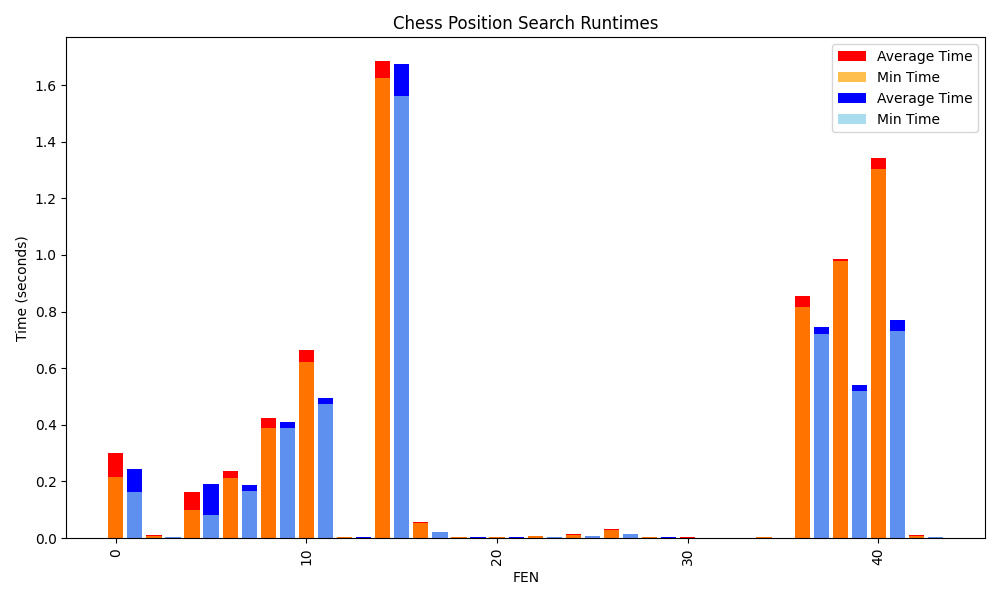
\includegraphics[width=1\linewidth]{cache-move-type.png}
    \caption{This show the speed up that we got from caching the move type in the Move class.}
    \label{fig:enter-label}
\end{figure}

\subsection{Parallelism}
The simplest way to parallelize the move search algorithm is at the top level.
Given a board state, we can get all of the moves in that state; then, in parallel, we can use the mini-max algorithm to find those that result in the best position for that player.
However, this might not be the most optimal solution, as Figure~\ref{fig:cpu-trace} shows. This Figure~\ref{fig:cpu-trace} shows the CPU utilization over a run of iterative deepening looking for the best move.
The dips in CPU usage are when we are close to finishing a depth and starting the next depth.
This happens because one of the branches of the search is taking longer to search.
We were bottle necked by the slowest-running move search.
\begin{figure}[H]
    \centering
    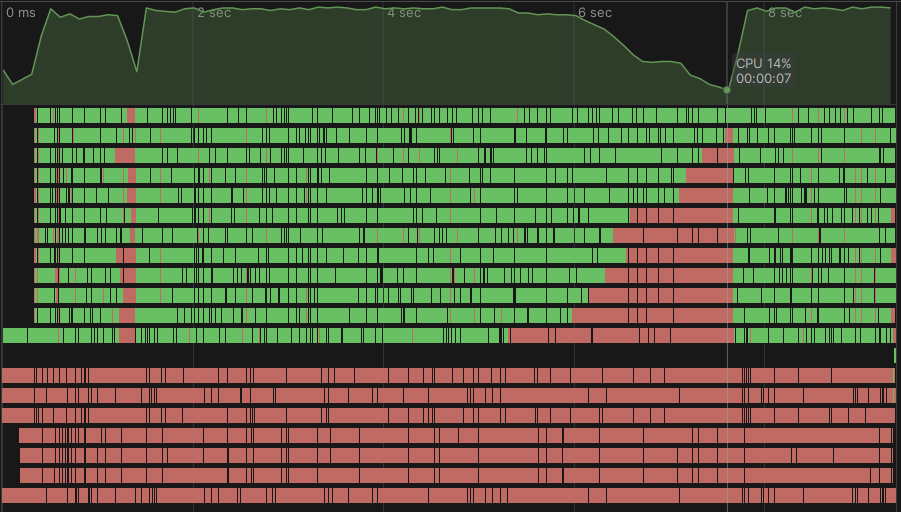
\includegraphics[width=1.0\linewidth]{parallism-cpu.png}
    \caption{Shows the usage of the CPU over the course of an execution of iterative deepening.}
    \label{fig:cpu-trace}
\end{figure}
We also do not always get the benefits of the parallelism.
For example, if there are only a few moves at depth one you do not get the benefits of parallelism.

\subsection{Piece Singletons}
This is a very simple idea that greatly reduces the number of objects that we need to make.
The idea is that you do not need to make multiple instances of a Piece (e.g. all of the white pawns in the entire program can point to the same Pawn object).
This greatly reduces the amount of time that we spend copying the board while branching.
Instead of allocating a new object we just need to copy the array of Piece references to the other board.
We can create all of the Piece classes with two static variables one for the white piece and one for the black piece.
A Piece with this schema becomes just a collection of functions.

\subsection{Alpha-Beta Pruning}
 Alpha-beta pruning is an optimization for the mini-max algorithm.
 It skips evaluating branches that will not affect the final optimal decision.
 It does this by using two values—alpha (best already explored path for the maximizer) and beta (best already explore path for the minimizer)—to "prune" unneeded branches.
 The following optimization relies on the fact that we are using alpha-beta pruning when we are looking for a move.

\subsubsection{Pseudo Move Generation}
This optimization relies on the benefits of alpha-b beta pruning.
The basic idea is that produce all of the valid move from any position is much more computationally expensive then generating a list of pseudo valid moves.
The moves are not valid in the sense that the computer is allowed to put itself in check.
This does not matter because, during the mini-max algorithm, the players would never choose to put themselves in check.
Furthermore, those branches will be quickly pruned because of alpha-beta pruning.

The reason that checking if a move puts the moving play in check is because it is implemented by copying the board preforming the move and check it the king is under attack.
This can be optimized by adding a conceptual adding an undo move function.
Adding this function is not as simple at first glance it requires adding some extra board state like the piece that was taken last.
It also requires updating other castling and enpassant variables.

One limitation of this approach is that the chess engine is very bad at finding checkmate.
It theoretically should be able to but I think that it does not find the right move because the player is consider moves that it is not able to make.

\subsubsection{Move Heuristic}
We were also able to give a value to move.
The value of the move is defined as the change in the eval of the board.
This allows us to sort the moves before they are searched to find the best move.
This allows us to more quickly look at the good moves and prune the bad moves.
However, it does introduce overhead that the list of moves needs to be sorted.
In some cases, the overhead was more than the benefits we got from pruning.
Defining a better heuristic could improve performance.

A possible better heuristic would be to use the evaluation of the board found in the previous runs of iterative deepening.
Since we are already computing those values we could cache them and use them in subsequent runs.
However, it is not guaranteed that a move at depth 4 would also be good at depth 5.
Though it could provide

 \begin{figure}[H]
     \centering
     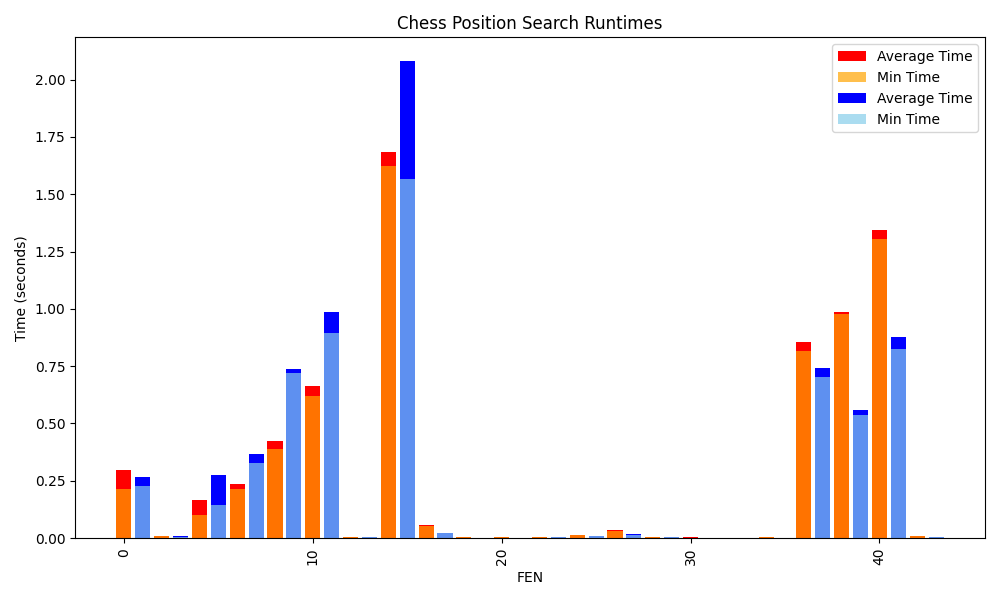
\includegraphics[width=1\linewidth]{sort.png}
     \caption{This shows the small benefits of the move heuristics had on performance. They should only increase with depth because it will be able to prune more.}
     \label{fig:enter-label}
 \end{figure}
\section{Results}
One simple bench that I would run throughout testing the application was how quickly we could count all the nodes from the start position.
When I first started it took 95 seconds to compute to a depth of 5 from the starting position.
We were able to reduce this to a speed of 5 seconds at the same depth.
This also does not consider the benefit of alpha-beta pruning when the engine is playing a game.

\subsection{Further Directions}
I experiment a little with using different versions of Java to compile and run the jar file on my system.
And though I was able to detect a different in runtime, I was not able to run a complete benchmark comparing the different version.
This would be a good place to spend time doing research.

Also one of the major bottlenecks of the program is copying the board state.
Using an idea similar to bit boards should be able to make this faster or a strategy I outlined in \ref{sec:board}.
I think that the problem is that I did not use the correct data structure.
The and, or, and shift operations were not optimized for the class I used, BigInteger.
Exploring other representations would be good future work.

It would also be good to add a new way of parallising the program because with the way it is implemented in the paper you do not get the benefits of alpha beta pruning at the base layer.
This is the most important place to have it because it will allow you to prune the largest branches.

A way to visualize the graph that was searched would also be very helpful for finding bugs in the evaluation function and search function.
This could be done with the Graphviz software.

Getting better hardware would also be a major help to performance (I am just running it on my laptop).

\begin{thebibliography}{99}

\bibitem{jones}
Peter Ellis Jones' Gist.
\url{https://gist.github.com/peterellisjones/8c46c28141c162d1d8a0f0badbc9cff9}

\bibitem{pgn}
PGN Mentor – Abdusattorov's Games.
\url{https://www.pgnmentor.com/players/Abdusattorov/}

\bibitem{lichess-bot}
Lichess Bot.
\url{https://github.com/lichess-bot-devs/lichess-bot}

\bibitem{uci}
UCI Protocol.
\url{https://www.chessprogramming.org/UCI}

\bibitem{fen}
Forsyth–Edwards Notation (FEN).
\url{https://www.chessprogramming.org/Forsyth-Edwards_Notation}

\bibitem{roce}
ROCE – Roman's Own Chess Engine.
\url{http://www.rocechess.ch/rocee.html}

\bibitem{parallel}
Parallel Alpha–Beta Search Discussion.
\url{https://stackoverflow.com/questions/26748118/is-it-possible-to-run-a-minimax-search-with-alpha-beta-pruning-in-parallel-with}

\bibitem{stockfish}
Stockfish Chess Engine.
\url{https://stockfishchess.org/}

\bibitem{stockwiki}
Stockfish Wikipedia Entry.
\url{https://en.wikipedia.org/wiki/Stockfish_(chess)#Competition_results}

\bibitem{bitboard}
Bitboards – Chess Programming Wiki.
\url{https://www.chessprogramming.org/Bitboards}

\bibitem{testing}
Testing a Chess Engine.
\url{https://www.royvanrijn.com/blog/2011/02/unit-testing-a-chess-engine/}

\end{thebibliography}

\section{Appendix}
In order to showcase the application we will show that the engine finds a checkmate that is at depth 5.
\begin{figure}[H]
    \centering
    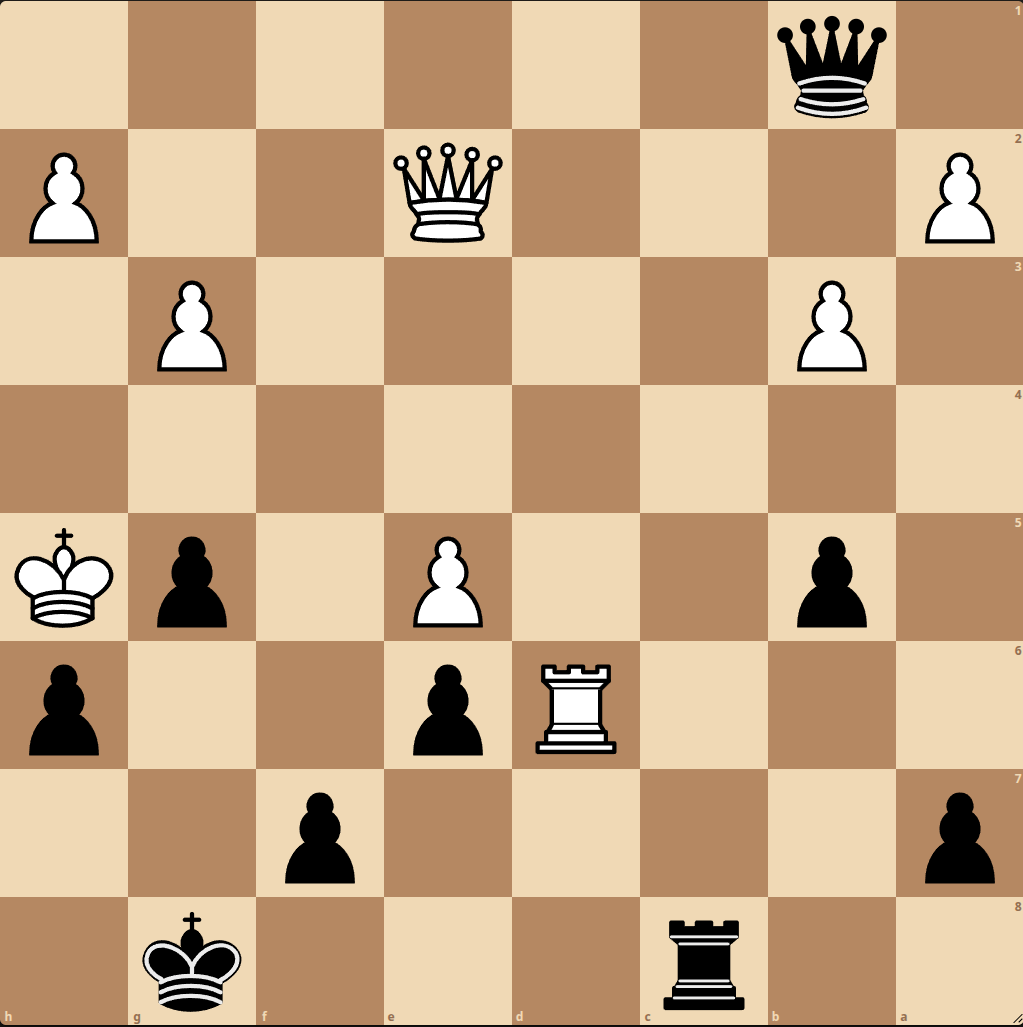
\includegraphics[width=0.7\linewidth]{appendix-board.png}
    \caption{Can you find mate in 5 moves. It is black turn to move.}
    \label{fig:enter-label}
\end{figure}

The chess engine was given the following fen string.
\begin{verbatim}
2r3k1/p4p2/3Rp2p/1p2P1pK/8/1P4P1/P3Q2P/1q6 b - - 0 1
\end{verbatim}
We then ran iterative deepening for 10-seconds.
You can see how long it took to compute each depth.
You can also notice that it was not able to finish depth 6 because it reached the 10 second timeout.
However, it would be ideal if the engine would return as soon as it found checkmate.
Regardless, it was able to find the first step of the checkmate sequence.
The solution is on the next page.

\begin{figure}[H]
    \centering
    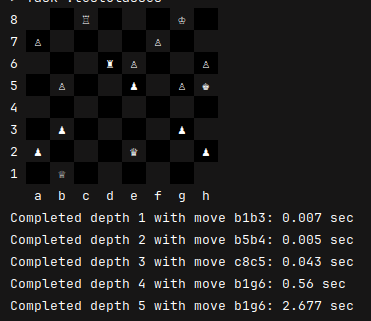
\includegraphics[width=1\linewidth]{output.png}
    \caption{Here is the output of the chess engine that ran iterative deepening for 10 seconds.}
    \label{fig:enter-label}
\end{figure}
You can view the solution here.
\url{https://lichess.org/analysis/standard/2r3k1/p4p2/3Rp2p/1p2P1pK/8/1P4P1/P3Q2P/1q6_b_-_-_0_1#2}

\subsection{Solution}
\begin{verbatim}
b1g6
h5g4
g6f5
g4h5
f5h3
\end{verbatim}

\end{document}
